% 2011 年陕西卷文科第 19 题：曲线 y=e^x 上点列 P_k、Q_k 与切线。
% 来源 PDF：普通高考/2011/2011陕西文.pdf，SHA-256 ae7984faa1d48b19525f0991a1795d8ea34b7ac65d9c067f4862c59ae112880e。
% 原页：第 2 页第 2 栏中部，书页码 696。示意。
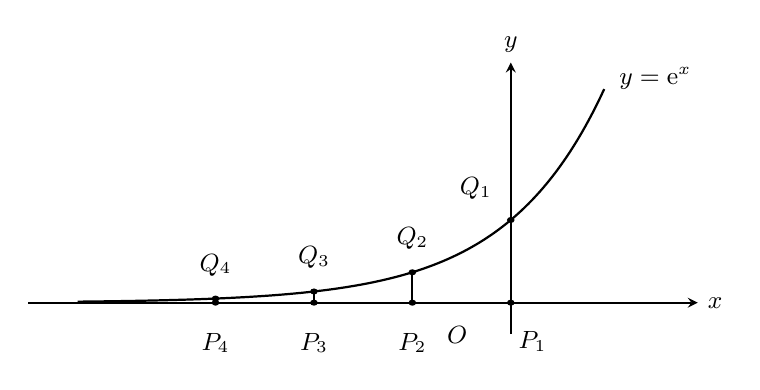
\begin{tikzpicture}[>=stealth, semithick, font=\small, xscale=1.25]
  \draw[->] (-4.9,0)--(1.9,0) node[right] {$x$};
  \draw[->] (0,-0.4)--(0,3.05) node[above] {$y$};
  \draw[thick, domain=-4.4:0.95, samples=140] plot (\x,{1.05*exp(\x)});
  \node[right] at (1.0,2.85) {$y=\mathrm e^x$};
  \foreach \k in {1,2,3,4} {
    \pgfmathsetmacro{\xk}{1-\k}
    \pgfmathsetmacro{\yk}{1.05*exp(\xk)}
    \draw[thick] (\xk,0)--(\xk,\yk);
    \fill (\xk,0) circle (1.1pt);
    \fill (\xk,\yk) circle (1.1pt);
    \ifnum\k=1\relax
      \node[below] at (0.22,-0.24) {$P_1$};
      \node[right] at (-0.62,1.45) {$Q_1$};
    \else
      \node[below] at (\xk,-0.26) {$P_{\k}$};
      \node[above] at (\xk,\yk+0.16) {$Q_{\k}$};
    \fi
  }
  \node[below left] at (-0.34,-0.18) {$O$};
\end{tikzpicture}
